%%%%%%%%%%%%%%%%%%%%%%%%%%%%%%%%%%%%%%%%%
% Developer CV
% LaTeX Template
% Version 1.0 (28/1/19)
%
% This template originates from:
% http://www.LaTeXTemplates.com
%
% Authors:
% Jan Vorisek (jan@vorisek.me)
% Based on a template by Jan Küster (info@jankuester.com)
% Modified for LaTeX Templates by Vel (vel@LaTeXTemplates.com)
%
% License:
% The MIT License (see included LICENSE file)
%
%%%%%%%%%%%%%%%%%%%%%%%%%%%%%%%%%%%%%%%%%
% https://www.latextemplates.com/template/developer-cv

%----------------------------------------------------------------------------------------
%	PACKAGES AND OTHER DOCUMENT CONFIGURATIONS
%----------------------------------------------------------------------------------------

\documentclass[9pt]{developercv} % Default font size, values from 8-12pt are recommended

\usepackage{svg}
\usepackage{xurl}
\usepackage{markdown}
\markdownSetup{
	renderers = {
		link = {%
			#1%
			% TODO: For some reason _ in url turn in _{}
			% \href{#2}{#1}%
		},
	},
}

%----------------------------------------------------------------------------------------

\begin{document}

\input{{{lang}}.tex}

%----------------------------------------------------------------------------------------
%	TITLE AND CONTACT INFORMATION
%----------------------------------------------------------------------------------------

\begin{minipage}[t]{0.45\textwidth} % 45% of the page width for name
	\vspace{-\baselineskip} % Required for vertically aligning minipages

	% If your name is very short, use just one of the lines below
	% If your name is very long, reduce the font size or make the minipage wider and reduce the others proportionately
	\colorbox{black}{{\HUGE\textcolor{white}{\texttt{\textbf{\MakeUppercase{Tim}}}}}} % First name

	\colorbox{black}{{\HUGE\textcolor{white}{\texttt{\textbf{\MakeUppercase{Huizinga}}}}}} % Last name

	\vspace{6pt}

	{\huge Applied Physics Student} % Career or current job title
\end{minipage}
\begin{minipage}[t]{0.275\textwidth} % 27.5% of the page width for the first row of icons
	\vspace{-\baselineskip} % Required for vertically aligning minipages

	% The first parameter is the FontAwesome icon name, the second is the box size and the third is the text
	% Other icons can be found by referring to fontawesome.pdf (supplied with the template) and using the word after \fa in the command for the icon you want
	\IfFileExists{latex/private.tex}{
		% File containing somewhat private information, not checked into the repository
		\input{latex/private.tex}

		\icon{\faMapMarker*}{12}{\City}\\
		\icon{\faPhone*}{12}{\Phone}\\
		\icon{\faAt}{12}{\href{mailto:\Email}{\texttt{\Email}}}\\
	}{
		\hfill
	}
\end{minipage}
\begin{minipage}[t]{0.275\textwidth} % 27.5% of the page width for the second row of icons
	\vspace{-\baselineskip} % Required for vertically aligning minipages

	% The first parameter is the FontAwesome icon name, the second is the box size and the third is the text
	% Other icons can be found by referring to fontawesome.pdf (supplied with the template) and using the word after \fa in the command for the icon you want
	\icon{\faGlobe}{12}{\href{https://huizinga.dev}{\texttt{huizinga.dev}}}\\
	\icon{\faGithub}{12}{\href{https://github.com/DreadedX}{\texttt{github.com/DreadedX}}}\\
	\icon{\faGit}{12}{\href{https://git.huizinga.dev/explore}{\texttt{git.huizinga.dev}}}\\
\end{minipage}

\vspace{0.5cm}

%----------------------------------------------------------------------------------------
%	INTRODUCTION
%----------------------------------------------------------------------------------------

\cvsect{\WhoAmI}

\begin{minipage}[t]{0.25\textwidth}
	\vspace{-\baselineskip} % Required for vertically aligning minipages

	\begin{tikzpicture}
		\clip (0,0)  circle (1.8cm) ;
		\node[anchor=center] at (0, -0.2) {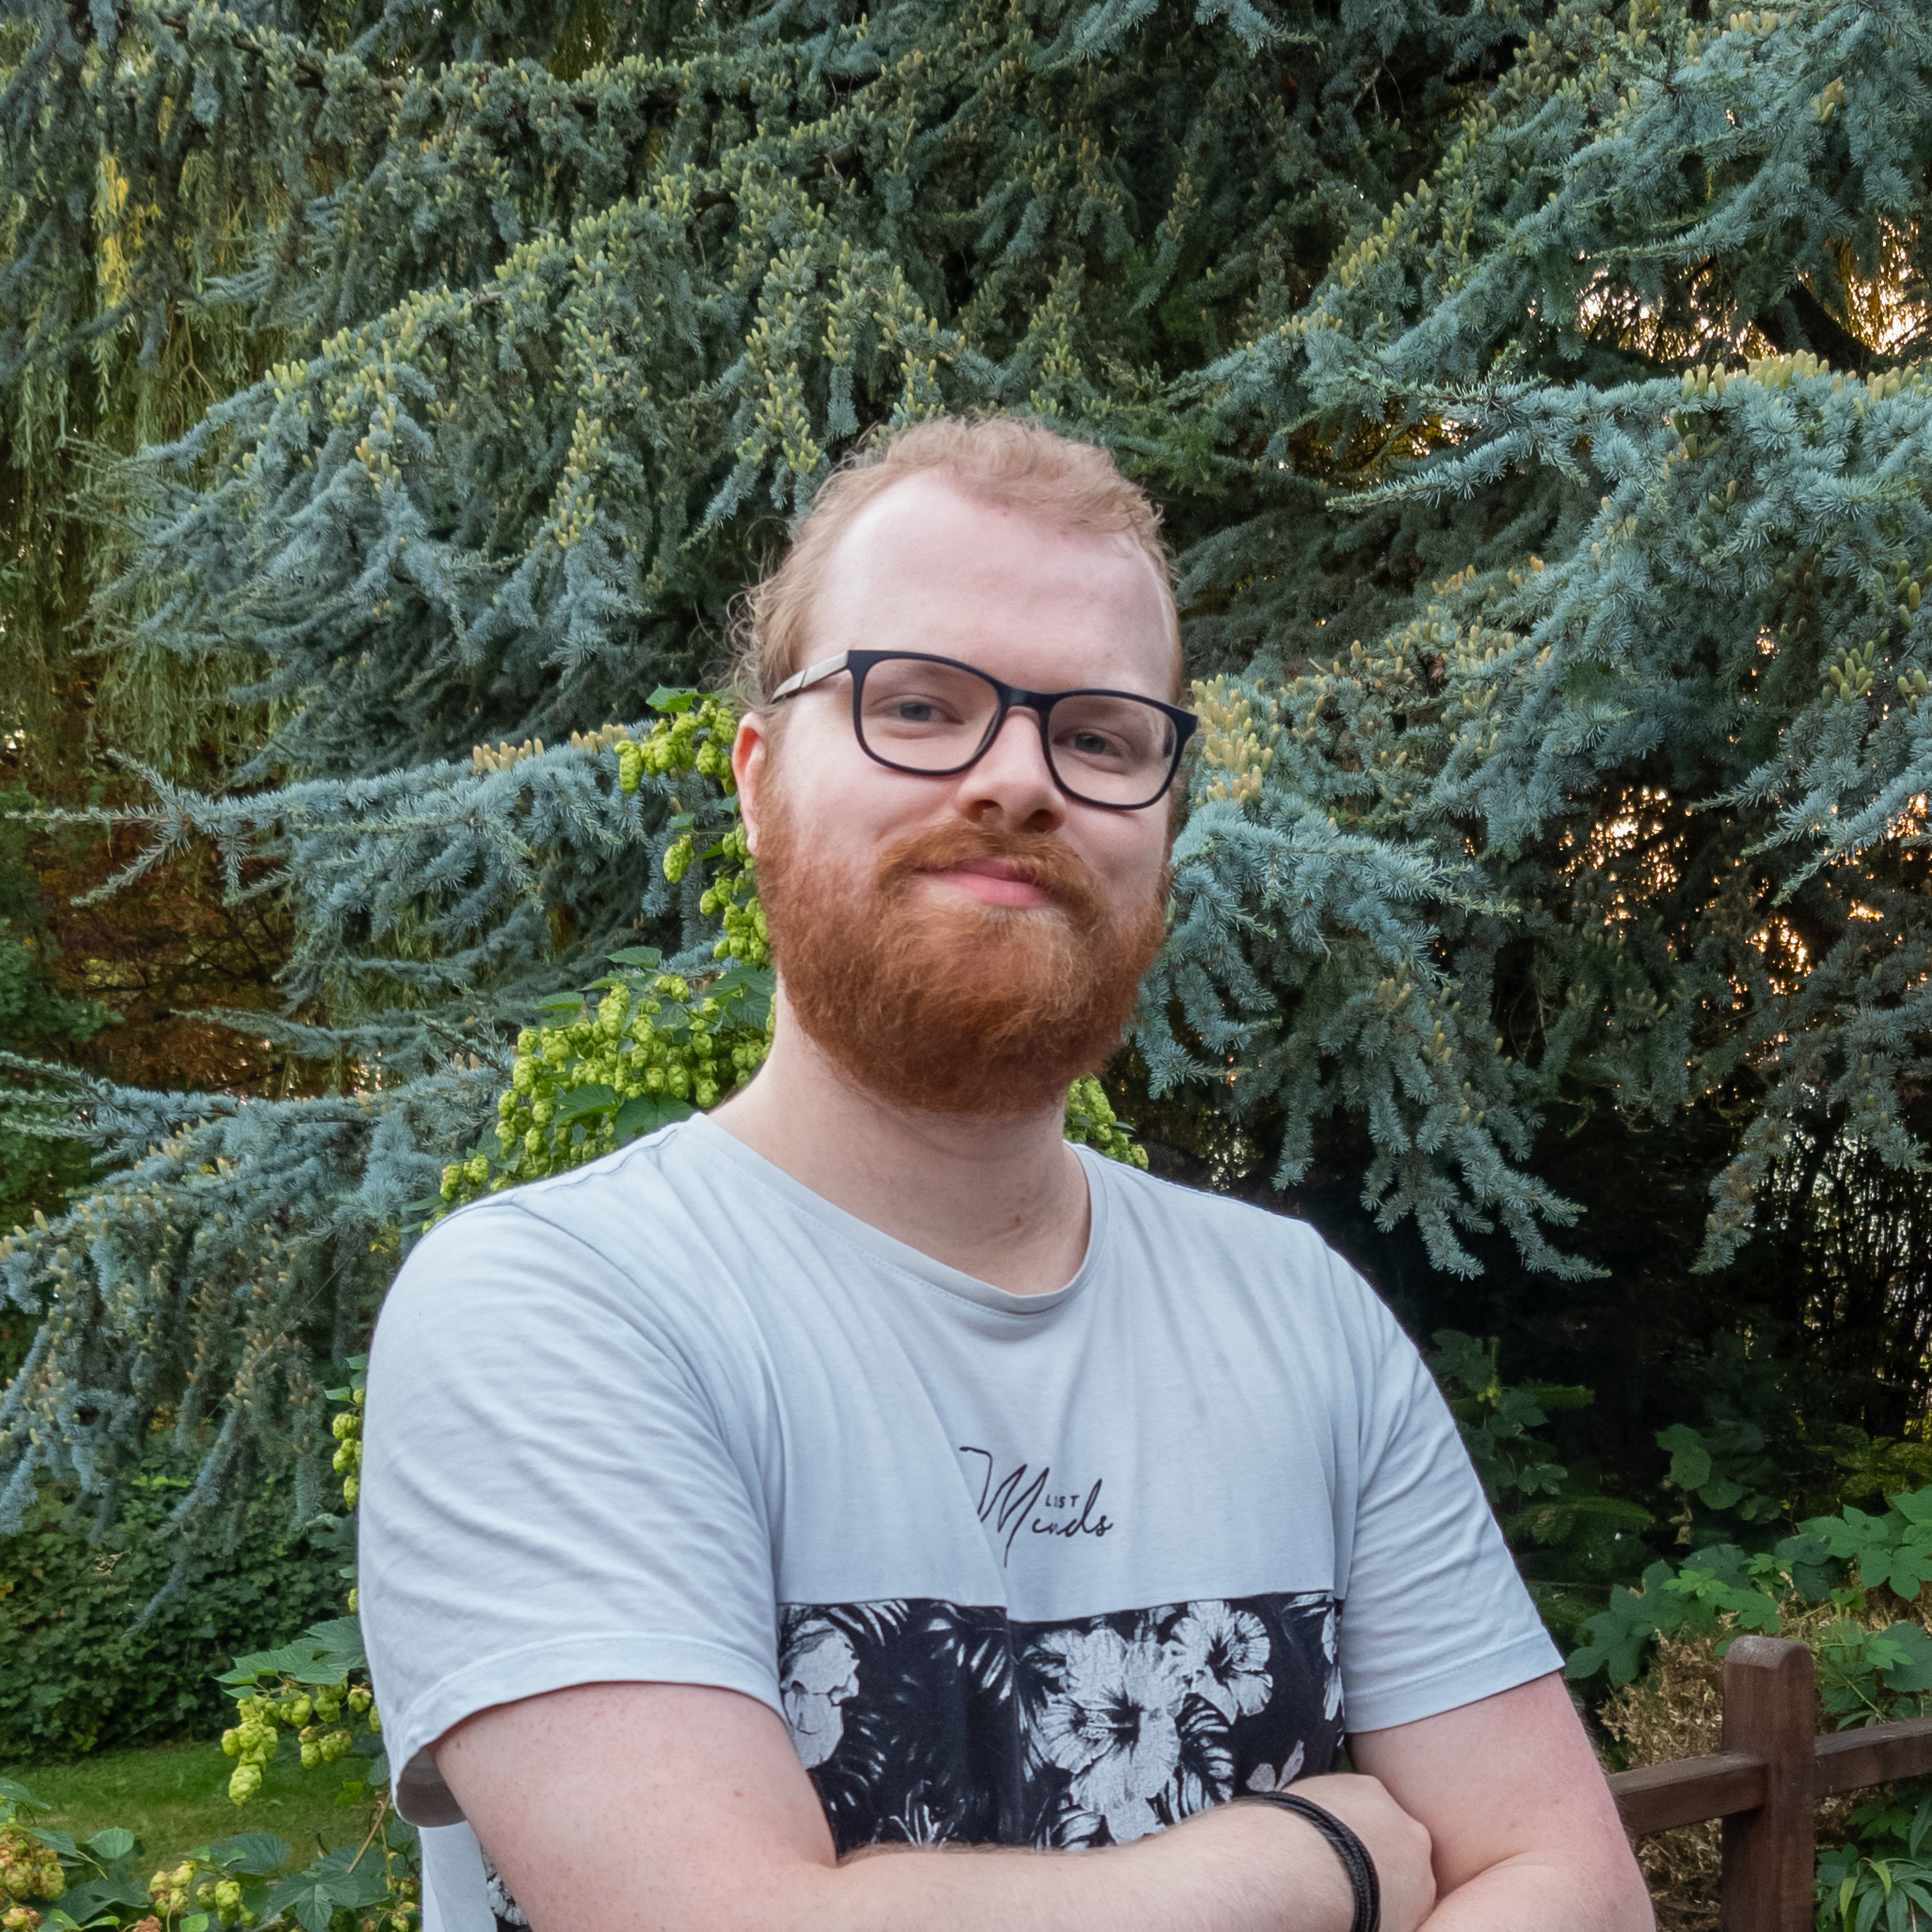
\includegraphics[width=6cm]{images/pfp.jpg}};
		%adjust this coordinate to move image
	\end{tikzpicture}
\end{minipage}
\begin{minipage}[t]{0.75\textwidth} % 40% of the page width for the introduction text
	\vspace{-\baselineskip} % Required for vertically aligning minipages

	\vspace{0.3cm}

	\input{latex/blurb.{{lang}}.md.tex}

\end{minipage}

%----------------------------------------------------------------------------------------
%	EXPERIENCE
%----------------------------------------------------------------------------------------

\cvsect{\Experience}

\begin{entrylist}
	\input{latex/experience.{{lang}}.yml.tex}
\end{entrylist}

%----------------------------------------------------------------------------------------
%	EDUCATION
%----------------------------------------------------------------------------------------

\cvsect{\Education}

\begin{entrylist}
	\input{latex/education.{{lang}}.yml.tex}
\end{entrylist}

%----------------------------------------------------------------------------------------
%	ADDITIONAL INFORMATION
%----------------------------------------------------------------------------------------

\begin{minipage}[t]{0.18\textwidth}
	\vspace{-\baselineskip} % Required for vertically aligning minipages

	\cvsect{\ProgrammingLanguages}

	\iconsvg{rust}{12}{Rust}\\
	\hfill
	\iconsvg{c}{12}{C}\\
	\hfill
	\iconsvg{javascript}{12}{JavaScript}\\
	\hfill
	\iconsvg{python}{12}{Python}\\
	\hfill
	\iconsvg{java}{12}{Java}\\
	\hfill
	\iconsvg{csharp}{12}{C\#}\\
\end{minipage}
\begin{minipage}[t]{0.18\textwidth}
	\vspace{-\baselineskip} % Required for vertically aligning minipages
	\vspace{32.35pt} % Make sure it lines up with the rest

	\iconsvg{cpp}{12}{C++}\\
	\hfill
	\iconsvg{go}{12}{Go}\\
	\hfill
	\iconsvg{typescript}{12}{TypeScript}\\
	\hfill
	\iconsvg{lua}{12}{Lua}\\
	\hfill
	\iconsvg{kotlin}{12}{Kotlin}\\
	\hfill
	\iconempty{12}{Verilog}\\
\end{minipage}
\hfill
\begin{minipage}[t]{0.18\textwidth}
	\vspace{-\baselineskip} % Required for vertically aligning minipages

	\cvsect{\OtherSkills}

	\icon{\faCalculator}{12}{\Maths}\\
	\hfill
	\iconsvg{linux}{12}{Linux}\\
	\hfill
	\iconsvg{git}{12}{Git}\\
	\hfill
	\iconsvg{android}{12}{Android Dev}\\
	\hfill
	\icon{\faMicrochip}{12}{Embedded}\\
	\hfill
	\iconempty{12}{\Soldering}\\
\end{minipage}
\begin{minipage}[t]{0.18\textwidth}
	\vspace{-\baselineskip} % Required for vertically aligning minipages
	\vspace{32.35pt} % Make sure it lines up with the rest

	\icon{\faApple*}{12}{\Physics}\\
	\hfill
	\iconsvg{bash}{12}{Bash}\\
	\hfill
	\iconsvg{docker}{12}{Docker}\\
	\hfill
	\iconsvg{latex}{12}{LaTeX}\\
	\hfill
	\iconempty{12}{PCB Design}\\
\end{minipage}
\hfill
\begin{minipage}[t]{0.18\textwidth}
	\vspace{-\baselineskip} % Required for vertically aligning minipages

	\cvsect{\Languages}

	\textbf{\Dutch} \\
	\hspace*{2em} \Native \\
	\textbf{\English} \\
	\hspace*{2em} \NearNative

	\vspace{8pt}

	\cvsect{\Hobbies}

	\AnalogPhotography\\
	\HouseMusic
\end{minipage}

%----------------------------------------------------------------------------------------
%	PROJECTS
%----------------------------------------------------------------------------------------

\clearpage
\begin{minipage}[t]{1\textwidth}
	\vspace{-\baselineskip} % Required for vertically aligning minipages

	\colorbox{black}{{\Huge\textcolor{white}{\textbf{\MakeUppercase{\Projects}}}}}
\end{minipage}

\vspace{8pt}

\begin{minipage}[t]{0.45\textwidth}
	\vspace{-\baselineskip} % Required for vertically aligning minipages
	\input{latex/project/automation.{{lang}}.md.tex}

	\vspace{6pt}

	\input{latex/project/z80.{{lang}}.md.tex}
\end{minipage}
\hfill
\begin{minipage}[t]{0.45\textwidth}
	\vspace{-\baselineskip} % Required for vertically aligning minipages
	\input{latex/project/car-stereo.{{lang}}.md.tex}

	\vspace{6pt}

	\input{latex/project/pico_p1.{{lang}}.md.tex}
\end{minipage}
\hfill

%----------------------------------------------------------------------------------------

\end{document}
